\documentclass[journal]{IEEEtran}
% IEEE Letters style (two-column journal). Compiles on Overleaf with pdfLaTeX + BibTeX.
% Every result number comes from generated/numbers.tex, written by
% scripts/make_paper_figures.py from results/context_study/context_runs.csv.

\usepackage{cite}
\usepackage{amsmath,amssymb}
\usepackage{graphicx}
\usepackage{booktabs}
\usepackage{xcolor}
\usepackage{tikz}
\usetikzlibrary{positioning,arrows.meta,fit,backgrounds}
\usepackage[hidelinks]{hyperref}

% Generated by scripts/make_paper_figures.py -- do not edit by hand.
\newcommand{\NumRuns}{720}
\newcommand{\NumSeeds}{10}
\newcommand{\PdrTrace}{99.8}
\newcommand{\PdrStress}{65.0}
\newcommand{\TelGain}{-3.5}
\newcommand{\TelLo}{-5.1}
\newcommand{\TelHi}{-2.1}
\newcommand{\MaskGain}{4.2}
\newcommand{\MaskLo}{2.2}
\newcommand{\MaskHi}{5.9}
\newcommand{\PrimGain}{-2.7}
\newcommand{\PrimLo}{-3.9}
\newcommand{\PrimHi}{-1.5}
\newcommand{\AccCcraStress}{46.0}
\newcommand{\AccMaskStress}{49.5}
\newcommand{\AccNoctxStress}{45.3}
\newcommand{\AccFltrustStress}{50.1}
\newcommand{\FltOverCcraStress}{4.1}
\newcommand{\TelIdeal}{-0.8}
\newcommand{\RejCcra}{41.2}
\newcommand{\RejMask}{13.8}
\newcommand{\AccptCcra}{8.8}
\newcommand{\AccptMask}{13.5}
\newcommand{\RejFltrust}{4.8}
\newcommand{\VsFltTrace}{2.6}
\newcommand{\VsFltTraceLo}{0.9}
\newcommand{\VsFltTraceHi}{4.5}
\newcommand{\VsFltStress}{-0.6}
\newcommand{\VsFltStressLo}{-2.0}
\newcommand{\VsFltStressHi}{1.0}
\newcommand{\DivFedavg}{41}
\newcommand{\DivMedian}{26}
\newcommand{\AllMask}{52.8}
\newcommand{\AllFedavg}{37.3}

\newcommand{\pp}{\,pp}
\newcommand{\ci}[2]{$[#1,\,#2]$}

\begin{document}

\title{Erasure-Aware Byzantine-Robust Aggregation for Hierarchical UAV-Swarm Federated Learning: When Link Telemetry Hurts}

\author{%
  First~Author, Second~Author, and Third~Author%
  \thanks{The authors are with the Department of Electronics and Communication Engineering,
  National Institute of Technology Warangal, Telangana 506004, India.}%
  \thanks{Code, data and the scripts that produce every figure in this letter:
  \url{https://github.com/sasank-555/uav-swarm-fl}.}%
}

\maketitle

\begin{abstract}
Federated learning (FL) lets a UAV swarm train a shared model without moving raw
sensor data, but tactical links lose packets and some UAVs may be compromised.
Byzantine-robust aggregation rules usually assume that every update arrives intact,
while channel-aware FL rarely assumes adversaries. We study a hierarchical UAV-swarm
FL system whose uplinks are driven by a measured air-to-ground received-power trace,
and a trusted-reference reputation aggregator with three levels of channel awareness:
none, packet-erasure masking, and full link telemetry (packet delivery ratio,
reliability, geometry, mobility and handover) inside the reputation update. In a
prespecified paired study of \NumRuns{} runs (\NumSeeds{} seeds, three model-poisoning
attacks, six aggregators), erasure masking raises accuracy under attack at a 5\,dB
link by \MaskGain\pp{} (95\% CI \ci{\MaskLo}{\MaskHi}), whereas adding telemetry
\emph{changes} it by $\TelGain$\pp{} (\ci{\TelLo}{\TelHi}), because it rejects
\RejCcra\% of honest updates. We trace this to an asymmetric reputation rule whose
stationary point drifts toward a UAV's worst rounds when its link is weak.
\end{abstract}

\begin{IEEEkeywords}
Federated learning, UAV swarm, Byzantine robustness, packet erasure, hierarchical aggregation, reputation.
\end{IEEEkeywords}

\section{Introduction}
\IEEEPARstart{U}{AV} swarms increasingly train perception models collaboratively,
and FL~\cite{mcmahan2017fedavg} keeps each UAV's imagery on board while exchanging
only model updates~\cite{xiao2021uavswarm}. Two impairments act on those updates at
once. First, air-to-ground links fade, hand over between base stations (BSs) and
miss deadlines, so updates arrive with missing packets~\cite{shirvanimoghaddam2022erroneous}.
Second, captured or spoofed UAVs can send poisoned updates. Robust rules such as
Krum~\cite{blanchard2017krum}, coordinate-wise median~\cite{yin2018median} and
FLTrust~\cite{cao2021fltrust} address the second problem but treat every received
vector as complete; channel-aware FL and anti-jamming designs~\cite{barkatsa2024jamming}
address the first but do not assume adversarial clients. Reputation-based defenses are
attractive for persistent swarm members, yet they can themselves be gamed~\cite{liu2026evade}.

A natural idea is to let the BS's own link telemetry modulate trust: a UAV on a
poor link should not be blamed for an update that \emph{looks} unusual because of
the channel. Our earlier single-seed experiments suggested such a context-calibrated
rule beat a cosine-weighted baseline taken from prior UAV-FL work~\cite{liao2023tee}.
This letter tests that idea under controlled conditions and finds that it does not hold.
The main contributions of this letter are as follows:
\begin{enumerate}
\item We model hierarchical UAV-swarm FL whose uplink packet erasures are driven by
  a measured DeepSense~6G UAV received-power trace~\cite{alkhateeb2023deepsense}, with
  BS association, handover and model-poisoning attackers.
\item We propose an erasure-aware reputation aggregator and isolate its two
  channel-aware mechanisms, erasure masking and telemetry-weighted reputation, in a
  prespecified, paired \NumRuns-run simulation study.
\item We derive the steady-state reputation of the update rule and show that it explains
  why telemetry lowers accuracy as the link weakens, while erasure masking raises it.
\end{enumerate}

The rest of this letter is arranged as follows. Section~\ref{sec:model} describes the
system model and Section~\ref{sec:method} the proposed aggregation.
Section~\ref{sec:analysis} analyses its reputation update at steady state.
Section~\ref{sec:results} presents simulation results, and Section~\ref{sec:conclusion}
concludes the letter.

\section{System Model}
\label{sec:model}
\begin{figure}[t]
\centering
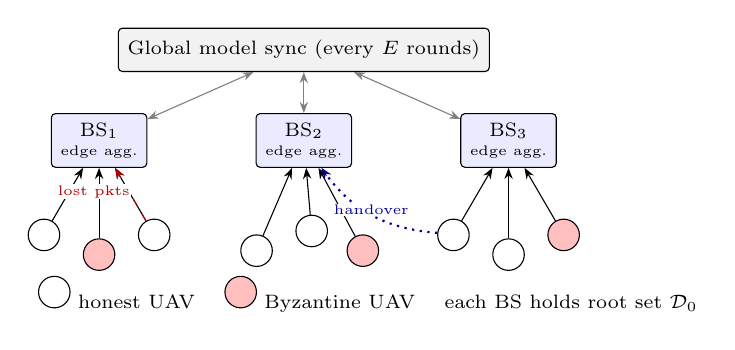
\begin{tikzpicture}[
  font=\scriptsize, >={Stealth[length=4pt]},
  bs/.style={draw, fill=blue!8, rounded corners=1.5pt, minimum width=11mm, minimum height=5mm, align=center},
  uav/.style={circle, draw, fill=white, inner sep=0pt, minimum size=4mm},
  bad/.style={uav, fill=red!25},
  cloud/.style={draw, fill=gray!10, rounded corners=1.5pt, minimum width=30mm, minimum height=5.5mm, align=center}]
  \node[cloud] (g) at (0,2.35) {Global model sync (every $E$ rounds)};
  \foreach \x/\n in {-2.6/1,0/2,2.6/3} {
    \node[bs] (b\n) at (\x,1.2) {BS$_\n$\\[-1pt]{\tiny edge agg.}};
    \draw[<->, gray] (b\n) -- (g);
  }
  \node[uav] (u1) at (-3.3,0) {};  \node[bad] (u2) at (-2.6,-0.25) {};  \node[uav] (u3) at (-1.9,0) {};
  \node[uav] (u4) at (-0.6,-0.2) {}; \node[uav] (u5) at (0.1,0.05) {};  \node[bad] (u6) at (0.75,-0.2) {};
  \node[uav] (u7) at (1.9,0) {};   \node[uav] (u8) at (2.6,-0.25) {};   \node[bad] (u9) at (3.3,0) {};
  \foreach \u/\b in {1/1,2/1,3/1,4/2,5/2,6/2,7/3,8/3,9/3} \draw[->] (u\u) -- (b\b);
  \draw[->, dashed, red!70!black] (u3) -- node[pos=0.55, left=-1pt, fill=white, inner sep=0.5pt] {\tiny lost pkts} (b1);
  \draw[->, dotted, thick, blue!60!black] (u7) to[bend left=25] node[pos=0.5, above=-1pt, fill=white, inner sep=0.5pt] {\tiny handover} (b2);
  \node[anchor=west] at (-3.5,-0.75) {\tikz\node[uav]{};~honest UAV \quad \tikz\node[bad]{};~Byzantine UAV \quad each BS holds root set $\mathcal{D}_0$};
\end{tikzpicture}
\caption{Hierarchical UAV-swarm FL: each BS aggregates the (partially received) updates
of the UAVs it serves; BS models are synchronized every $E$ rounds.}
\label{fig:system}
\end{figure}

\subsection{Hierarchical learning}
$K$ UAVs train a model $\mathbf{w}\in\mathbb{R}^P$ and are served by $B$ BSs
(Fig.~\ref{fig:system}). In round $t$, UAV $k$ attached to BS $b$ starts from the
edge model $\mathbf{w}_b^{t}$, runs local SGD on its private data $\mathcal{D}_k$ and
uploads $\boldsymbol{\Delta}_k^t$. BS $b$ aggregates the updates it receives into
$\mathbf{w}_b^{t+1}=\mathbf{w}_b^{t}+\mathrm{Agg}(\cdot)$. Every $E$ rounds the BS
models are averaged, weighted by each cell's number of training samples, and broadcast. Each BS also holds a
small trusted root set $\mathcal{D}_0$, disjoint from all UAV data, on which it
computes a reference update $\mathbf{r}_b^t$ each round, as in FLTrust~\cite{cao2021fltrust}.

\subsection{Erasure channel}
An update is split into packets of $L$ parameters. The uplink SNR $\gamma_k^t$ of UAV
$k$ is obtained by replaying a measured UAV received-power sequence~\cite{alkhateeb2023deepsense}
around an assumed reference SNR $\bar\gamma$ and adjusting it for the 3-D distance to
each virtual BS. Each packet is lost independently with probability
\begin{equation}
  p_k^t = \bigl(1+\exp\bigl(a(\gamma_k^t-\gamma_{\mathrm{th}})\bigr)\bigr)^{-1},
\end{equation}
and an update that misses the round deadline is dropped. The BS therefore observes
$\tilde{\boldsymbol\Delta}_k=\mathbf{m}_k\odot\boldsymbol\Delta_k$, where
$\mathbf{m}_k\in\{0,1\}^P$ marks delivered coordinates. Association uses a
hysteresis-and-time-to-trigger handover rule on received power.

\subsection{Threat model}
A fixed set of $f$ UAVs is Byzantine. They follow the protocol but replace their
update by a sign-flip ($-\lambda\boldsymbol\Delta_k$), an ALIE-style
update~\cite{baruch2019alie} ($\boldsymbol\mu - z\boldsymbol\sigma\odot\mathrm{sign}(\boldsymbol\mu)$,
from the honest updates of the same cell), or an inner-product-manipulation (IPM)
update~\cite{xie2019ipm} ($-\epsilon\boldsymbol\mu$). The ALIE and IPM attackers observe
honest updates in their cell, a deliberately strong assumption. Telemetry is measured
by the BS and is assumed authentic.

\section{Proposed Erasure-Aware Reputation Aggregation}
\label{sec:method}
Let $\mathcal{S}(\mathbf{x};\mathbf{m})$ restrict $\mathbf{x}$ to the coordinates where
$\mathbf{m}=1$. Each BS runs the following steps (index $t$ dropped).

\emph{1) Clipping.} With $\rho_k$ the RMS of the delivered entries of
$\tilde{\boldsymbol\Delta}_k$, scale the update by $s_k=\min(1,\mathrm{med}_j\,\rho_j/\rho_k)$.

\emph{2) Masked similarity.} Compare each update with the root update on delivered
coordinates only, so lost packets do not make an honest update look dissimilar:
$c_k=\cos\bigl(\mathcal{S}(s_k\tilde{\boldsymbol\Delta}_k;\mathbf{m}_k),\mathcal{S}(\mathbf{r};\mathbf{m}_k)\bigr)$.

\emph{3) Behavior score.} $b_k=\mathrm{clip}\bigl(c_k/\mathrm{med}_{j:c_j>0}\,c_j,\,0,\,1\bigr)$.

\emph{4) Reputation.} With memory $\beta$,
\begin{equation}
  T_k \leftarrow T_k + \eta_k\,(b_k-T_k),\qquad
  \eta_k=\begin{cases}(1-\beta)\,e_k, & b_k>T_k,\\ 1-\beta, & b_k\le T_k,\end{cases}
  \label{eq:rep}
\end{equation}
so that bad behavior is penalized at full rate and a weak link cannot shield an
attacker that drops its own packets. The \emph{evidence} $e_k\in[0,1]$ slows rewards
on poor links:
$e_k=\mathrm{PDR}_k\cdot R_k\cdot h_k\cdot g_k\cdot v_k$, the product of the packet
delivery ratio, long-term reliability, a handover penalty ($h_k=0.5$ during a
handover), a distance factor and a speed factor.

\emph{5) Masked weighted average.} UAVs with $T_k<\tau$ get zero weight; otherwise
$\omega_k=n_kT_k$, with $n_k=|\mathcal{D}_k|$ and a staleness discount. Each coordinate
is averaged only over the UAVs that delivered it:
\begin{equation}
  \mathrm{Agg}_p=\frac{\sum_k \omega_k\, m_{k,p}\, s_k\tilde\Delta_{k,p}}{\sum_k \omega_k\, m_{k,p}}.
\end{equation}

\emph{Variants.} \textbf{CCRA (full)} uses all steps with telemetry evidence $e_k$.
\textbf{Mask-only} sets $e_k=1$ but keeps the masks. \textbf{No-context} additionally sets
$\mathbf{m}_k=\mathbf{1}$, so lost packets enter steps 1--5 as zeros, which is how a
channel-unaware server sees them. (The SINR calibration of $c_k$ in our code is inactive
here because the study has no residual parameter noise, so the full-versus-mask-only
contrast isolates $e_k$.)

\section{Steady-State Analysis of the Reputation}
\label{sec:analysis}
Consider one UAV whose evidence is constant, $e_k=e\in(0,1]$, and whose behavior
scores $b\in[0,1]$ are i.i.d.\ with $\mathbb{E}[b]>0$. By~\eqref{eq:rep}, the
expected reputation step from level $T$ is $(1-\beta)\,g_e(T)$ with
\begin{equation}
  g_e(T)=e\,\mathbb{E}\bigl[(b-T)^+\bigr]-\mathbb{E}\bigl[(T-b)^+\bigr].
  \label{eq:drift}
\end{equation}

\emph{Proposition 1:} $g_e$ has a unique root $T^\star(e)\in(0,1)$, the steady state of
the mean reputation dynamics. $T^\star(1)=\mathbb{E}[b]$, $T^\star(e)$ is increasing in
$e$, and $T^\star(e)\to\operatorname{ess\,inf} b$ as $e\to0$.

\emph{Proof:} $g_e$ is continuous and strictly decreasing in $T$, with
$g_e(0)=e\,\mathbb{E}[b]>0$ and $g_e(1)=-\mathbb{E}[1-b]<0$, so the root exists and is
unique. For $e=1$, $g_1(T)=\mathbb{E}[b]-T$. Since $\partial g_e/\partial e=
\mathbb{E}[(b-T)^+]\ge0$ while $g_e$ decreases in $T$, the root rises with $e$. As
$e\to0$, $g_e(T)\to-\mathbb{E}[(T-b)^+]$, which is negative for every
$T>\operatorname{ess\,inf}b$. \hfill$\blacksquare$

The asymmetry intended to stop packet-dropping attackers therefore has a side
effect. An honest UAV with non-IID data has noisy scores, and on a weak link (small
$e$) its reputation settles near its \emph{worst} rounds instead of its average,
so it falls below the gate $\tau$ more often. An attacker's scores are already near
zero, so a smaller $e$ adds little suppression. Section~\ref{sec:results} tests this
prediction.

\section{Simulation Results}
\label{sec:results}

\subsection{Simulation Setup}
Table~\ref{tab:params} lists the values assumed for the parameters. Attackers are
chosen per seed and kept fixed across methods. The channel is either ideal or the
same measured trace replayed at $\bar\gamma=15$\,dB (mean PDR \PdrTrace\%) and at
$\bar\gamma=5$\,dB (mean PDR \PdrStress\%). The baselines are
FedAvg~\cite{mcmahan2017fedavg}, coordinate-wise median~\cite{yin2018median} and
FLTrust~\cite{cao2021fltrust}, the last given the same root set and a comparable
local-step budget.

\begin{table}[t]
\centering
\caption{Values Assumed for the Parameters}
\label{tab:params}
\footnotesize
\begin{tabular}{@{}p{0.5\columnwidth}p{0.45\columnwidth}@{}}
\toprule
Parameter & Value \\
\midrule
UAVs $K$; BSs $B$; attackers $f$; sync $E$ & 10; 3; 3; 5 \\
Rounds; local training & 100; one SGD epoch \\
Model & CNN, 156k parameters \\
Data & aerial CIFAR-10, Dirichlet($0.5$)~\cite{hsu2019noniid} \\
Root set $|\mathcal{D}_0|$; $\beta$; $\tau$ & 500 images; 0.5; 0.3 \\
Packet size $L$; $a$; $\gamma_{\mathrm{th}}$ & 1024; 1; 3\,dB \\
Reference SNR $\bar\gamma$ & ideal, 15\,dB, 5\,dB \\
Sign flip $\lambda$; ALIE $z$; IPM $\epsilon$ & 5; 1.5; 0.5 \\
Seeds; runs & \NumSeeds; \NumRuns{} \\
\bottomrule
\end{tabular}
\end{table}

The full factorial design crosses six aggregators, four attack settings (including
clean), three channels and \NumSeeds{} paired seeds. A run that diverges numerically
is scored at chance (10\%), never discarded. The primary contrast, CCRA minus
mask-only at 5\,dB minus the same at 15\,dB, and its 1\pp{} decision threshold were
fixed before the runs. Intervals are 95\% percentile bootstraps over seeds (10{,}000
resamples). All other contrasts are exploratory and not adjusted for multiple
comparisons.

\begin{figure}[t]
\centering
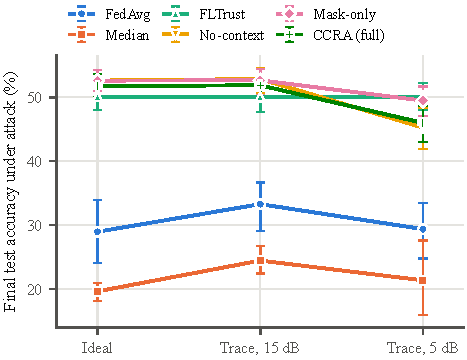
\includegraphics[width=\columnwidth]{figures/accuracy_vs_channel.pdf}
\caption{Final accuracy under attack (mean of sign-flip, ALIE and IPM over
\NumSeeds{} seeds; bars: 95\% bootstrap CI). Diverged runs count as 10\%.}
\label{fig:acc}
\end{figure}

\begin{table}[t]
\centering
\caption{Run outcomes over all \NumRuns{} runs (120 per method)}
\label{tab:outcomes}
\begin{tabular}{@{}lccc@{}}
\toprule
Method & Diverged & All runs (\%) & Attacked, 5\,dB (\%) \\
\midrule
FedAvg & 41/120 & 37.3 & 29.4 \\
Median & 26/120 & 29.3 & 21.3 \\
FLTrust & 0/120 & 50.6 & \textbf{50.1} \\
No-context & 0/120 & 51.4 & 45.3 \\
Mask-only & 0/120 & \textbf{52.8} & 49.5 \\
CCRA (full) & 0/120 & 51.1 & 46.0 \\
\bottomrule
\end{tabular}

\end{table}

\subsection{Robustness and Stability}
Fig.~\ref{fig:acc} and Table~\ref{tab:outcomes} show
that FedAvg and the coordinate-wise median diverged in \DivFedavg{} and \DivMedian{} of
their 120 runs respectively, whereas no root-referenced method (FLTrust and all three
CCRA variants) diverged. The median is likely fragile here because each cell holds only a few UAVs, so a
single attacker in a cell can already move the median. Across all runs,
mask-only attains the highest accuracy (\AllMask\% versus \AllFedavg\% for FedAvg).
Against FLTrust it gains \VsFltTrace\pp{} (\ci{\VsFltTraceLo}{\VsFltTraceHi}) under
attack at 15\,dB, but at 5\,dB the two are indistinguishable
($\VsFltStress$\pp, \ci{\VsFltStressLo}{\VsFltStressHi}; exploratory).

\begin{figure}[t]
\centering
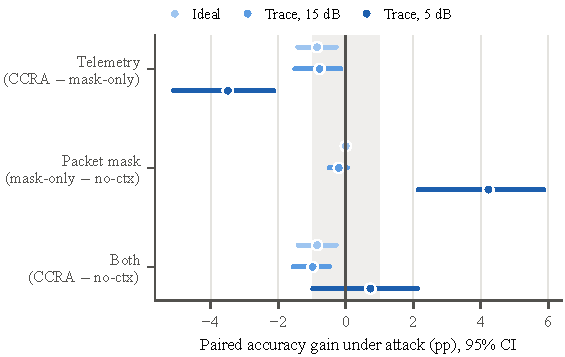
\includegraphics[width=\columnwidth]{figures/ablation_contrasts.pdf}
\caption{Paired ablation contrasts under attack. The gray band marks the
prespecified $\pm1$\pp{} region of practical equivalence.}
\label{fig:ablation}
\end{figure}

\subsection{Which Channel Awareness Helps}
Fig.~\ref{fig:ablation} separates the two
mechanisms. On the ideal channel the masks are all ones, so mask-only and no-context
coincide. As delivery degrades, erasure masking becomes valuable: at 5\,dB it adds
\MaskGain\pp{} (\ci{\MaskLo}{\MaskHi}). Telemetry does the opposite. At 5\,dB, full
CCRA minus mask-only is $\TelGain$\pp{} (\ci{\TelLo}{\TelHi}; \AccCcraStress\% versus
\AccMaskStress\%), and the prespecified interaction lies entirely below $-1$\pp.
Combining the two mechanisms leaves an inconclusive net effect relative to no-context.

\begin{figure}[t]
\centering
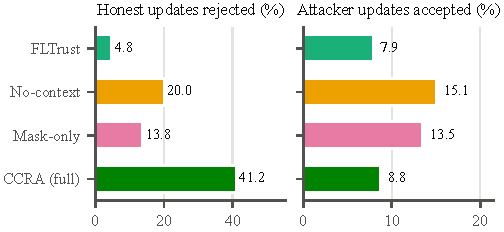
\includegraphics[width=\columnwidth]{figures/gate_rates.pdf}
\caption{Reputation-gate decisions under attack at 5\,dB, averaged over attacks and
seeds (percent of received updates).}
\label{fig:gate}
\end{figure}

\subsection{Validation of the Steady-State Analysis}
Fig.~\ref{fig:gate} matches Proposition~1. With telemetry, the
gate rejects \RejCcra\% of honest updates versus \RejMask\% for mask-only, and admits
only slightly fewer attacker updates (\AccptCcra\% versus \AccptMask\%). The rule
trades a small gain in attacker filtering for a large loss of honest data, and the
loss grows as the link weakens, where honest data is already scarce. FLTrust, which
has no memory, rejects only \RejFltrust\% of honest updates, consistent with its
resilience at 5\,dB. These rates are descriptive and support, but do not prove, the
causal account.

\subsection{Limitations}
The trace comes from one measured BS with virtual neighbors, the
SNR anchors are assumptions rather than calibrated values, the run includes few
handovers, and we use one dataset and model. Telemetry spoofing and adaptive attacks
on the reputation itself~\cite{liu2026evade} are not tested.

\section{Conclusion}
\label{sec:conclusion}
In a hierarchical UAV-swarm FL system with measured-trace packet erasures, the
channel-aware component that pays off is simple: compare and average each update
only on the coordinates that actually arrived. Feeding link telemetry into an
asymmetric reputation update looked reasonable but measurably hurt accuracy on weak
links by suppressing honest UAVs. Future work will redesign the reward rule so that
weak links do not bias reputation downward, evaluate it on fresh seeds and
higher-mobility traces, and study adaptive and telemetry-spoofing attackers.

\bibliographystyle{IEEEtran}
\bibliography{refs}

\end{document}
